%==============================================================================
%  Workshop No. 1 - Project Definition Report
%  Volcanic Activity Monitoring System (United States)
%  Team 6 - Data Analysis Programming 2026-II
%  Universidad Distrital Francisco Jose de Caldas
%
%  Build:  pdflatex project_definition.tex   (run twice for the ToC and references)
%  Images: docs/architecture.png and docs/er_diagram.png (rendered from the .mmd files)
%  Requires TeX Live 2020 or newer: the file name er_diagram.png contains an
%  underscore, which older distributions reject inside \includegraphics.
%==============================================================================
\documentclass[11pt,a4paper]{article}

\usepackage[utf8]{inputenc}
\usepackage[T1]{fontenc}
\usepackage[english]{babel}
\usepackage{lmodern}
\usepackage{textcomp}
\usepackage[a4paper,margin=2.3cm]{geometry}
\usepackage{amsmath}
\usepackage{graphicx}
\usepackage{booktabs}
\usepackage{longtable}
\usepackage{array}
\usepackage{caption}
\usepackage{enumitem}
\usepackage{xcolor}
\usepackage{listings}
\usepackage{fancyhdr}
\usepackage[hidelinks]{hyperref}

\graphicspath{{.}{docs/}{../docs/}}

\hypersetup{
  pdftitle={Workshop 1 - Volcanic Activity Monitoring: Project Definition Report},
  pdfauthor={Team 6 - Universidad Distrital Francisco Jose de Caldas},
  pdfsubject={Data Analysis Programming 2026-II, Workshop No. 1}
}

\captionsetup{font=small,labelfont=bf}
\setlist[itemize]{itemsep=2pt,topsep=3pt}
\setlist[enumerate]{itemsep=2pt,topsep=3pt}

\pagestyle{fancy}
\fancyhf{}
\lhead{\small Workshop 1 --- Volcanic Activity Monitoring}
\rhead{\small Team 6}
\cfoot{\thepage}
\renewcommand{\headrulewidth}{0.4pt}

\newcolumntype{L}[1]{>{\raggedright\arraybackslash}p{#1}}

\lstdefinestyle{evidence}{
  basicstyle=\scriptsize\ttfamily,
  breaklines=true,
  breakatwhitespace=false,
  columns=flexible,
  frame=single,
  framesep=4pt,
  rulecolor=\color{gray!50},
  backgroundcolor=\color{gray!8},
  showstringspaces=false,
  xleftmargin=0pt,
  aboveskip=6pt,
  belowskip=6pt
}
\lstset{style=evidence}

\title{\vspace{-1.2cm}\textbf{Workshop 1 --- Volcanic Activity Monitoring}\\[0.3em]
       \large Project Definition Report\\[0.2em]
       \normalsize Hazard Definition, Source Validation and Data Contract}

\author{%
  \textbf{Team 6}\\[0.4em]
  \begin{tabular}{ll}
    20231020006 & Juan Sebasti\'an Rangel Pinto\\
    20231020055 & Jhonatan David Vergara Jim\'enez\\
    20231020064 & Juli\'an Pulido\\
  \end{tabular}\\[0.8em]
  Computer Engineering Program --- School of Engineering\\
  Universidad Distrital Francisco Jos\'e de Caldas\\[0.3em]
  \small Professor: Eng. Carlos Andr\'es Sierra, M.Sc.
}
\date{Semester 2026-II \\[0.2em]
      \small Evidence retrieved 2026-11-10 and 2026-11-11}

%==============================================================================
\begin{document}
\maketitle
\thispagestyle{fancy}

\begin{abstract}
\noindent
This report formalises the semester project of Team~6: a multi-source ingestion and
analysis system for \textbf{volcanic activity in the United States}. It defines the
hazard and its severity measures, documents and validates four data sources with real
responses, profiles them, establishes the canonical mapping and the ingestion
contract, and defines the functional user, the user stories, a preliminary
\emph{Volcano Activity Indicator} (VAI) and the project risks. Every figure quoted
here was measured on responses retrieved on 2026-11-10 and 2026-11-11 and kept
unmodified under \texttt{workshop\_1/samples/}; the profiling notebook
\texttt{notebooks/01\_source\_profiling.ipynb} was executed top to bottom on
2026-11-11. The indicator of Section~\ref{sec:indicator} is a \textbf{monitoring and
correlation aid and is not an eruption forecast}.
\end{abstract}

\tableofcontents
\bigskip

%==============================================================================
\section{Project Overview}
\label{sec:overview}

\paragraph{Title.}
Volcanic Activity Monitoring System --- a multi-source ingestion and analysis pipeline
for the volcanoes of the United States.

\paragraph{Motivation.}
The United States has 165 Holocene volcanoes in the Smithsonian GVP catalogue, from
the Aleutians to Hawaii and the Cascades. The information about them is spread across
separate products: GVP keeps the eruption history, the USGS Hazard Notification
System (HANS) publishes the official alert level and aviation colour code, and the
USGS earthquake catalogue holds the seismicity. No single open product puts a
volcano's current alert, its recent nearby seismicity and its eruption history side by
side. An analyst who wants to answer \emph{``is this volcano behaving unusually right
now, compared with its own history?''} must open at least three systems and reconcile
three identifier conventions by hand. That reconciliation is the engineering problem
this project solves.

\paragraph{Goal.}
\begin{description}[style=nextline,leftmargin=0.5cm]
  \item[Data-engineering perspective] Integrate two historical sources (GVP Volcanoes
  of the World, USGS FDSN catalogue) and two incremental sources (USGS HANS, USGS
  real-time earthquake feed) into one canonical PostgreSQL/PostGIS model, with
  idempotent historical loading and watermark-based incremental ingestion.
  \item[Analytical perspective] Compare each volcano's current situation with its own
  historical baseline and summarise it in a Volcano Activity Indicator (VAI).
\end{description}

\paragraph{Scope.}
\begin{itemize}
  \item \textbf{Volcanoes:} the 165 GVP Holocene volcanoes with
  \texttt{Country = 'United States'} (Alaska, Hawaii, the Cascades, California, the
  Northern Mariana Islands and American Samoa), plus the HANS-monitored volcanoes that
  GVP keeps outside its Holocene list, for example Yellowstone (325010) and Long Valley
  Caldera (323822).
  \item \textbf{Eruptions:} the full Holocene record is loaded; time-series analysis
  starts in 1960.
  \item \textbf{Earthquakes:} 2010-01-01 to today, M~$\geq$~1.0, within 30~km of a
  volcano.
  \item \textbf{Current situation:} the current HANS alert level and colour code of
  each volcano, plus the last 7~days of nearby seismicity.
\end{itemize}

\paragraph{Explicit exclusions.}
\begin{itemize}
  \item No eruption forecasting or probability of eruption. The VAI is a monitoring and
  correlation aid.
  \item No volcanoes outside the United States. Non-US items of the weekly report are
  skipped.
  \item No gas emissions, deformation (InSAR/GNSS), thermal satellite data or
  ash-dispersion models.
  \item No scraping of the HTML weekly-report archive. GDACS is documented but
  disabled.
\end{itemize}

\paragraph{Constraints.}
Free and open sources only, with no API keys. Everything runs locally in Docker
Compose on student laptops. HANS returns only the latest notice per volcano, so the
alert history in the database starts with the first poll. The seismic component of the
indicator is relative to each volcano's own baseline. The system must expose the
command-line contract
\texttt{python ingest.py -{}-mode historical | incremental | status}, and running
either mode twice must not create duplicate rows. All documentation is in English and
no credential is committed to the repository.

%==============================================================================
\section{Hazard Definition}
\label{sec:hazard}

\paragraph{Phenomenon.}
A volcanic eruption is the release of magma, gas or fragmented rock at the surface.
Eruptions are usually preceded and accompanied by \emph{unrest}, which includes
earthquakes caused by magma and fluids moving under the volcano. Monitoring therefore
tracks two things: what the volcano is doing now (official alert level, observatory
notices) and how unusual that is for that volcano (its eruption history and normal
seismicity). The distinction matters for the data model: an eruption is an event,
unrest is a state.

Volcanic hazard also has two audiences with different time scales. Ground hazards
(lava flows, lahars, pyroclastic density currents) threaten the population around the
volcano; ash in the atmosphere threatens aviation hundreds of kilometres away. For
that reason the USGS publishes two independent scales for the same volcano.

\paragraph{Severity measures.}
Each event type keeps its own scale (Table~\ref{tab:severity}). No conversion between
them is attempted.

\begin{table}[h]
\centering
\small
\setlength{\tabcolsep}{4pt}
\caption{Severity measures handled by the system, with their units and sources.}
\label{tab:severity}
\begin{tabular}{@{}L{2.4cm}L{3.0cm}L{7.2cm}L{2.6cm}@{}}
\toprule
\textbf{Event type} & \textbf{Severity measure} & \textbf{Unit / scale} & \textbf{Source} \\
\midrule
Alert notice & USGS Volcano Alert Level + Aviation Colour Code &
Ordinal ground-hazard level: 1 NORMAL, 2 ADVISORY, 3 WATCH, 4 WARNING. Colour code
GREEN / YELLOW / ORANGE / RED (aviation hazard), kept as an attribute &
USGS HANS \\
\addlinespace
Eruption & Volcanic Explosivity Index (VEI) &
0--8, dimensionless, logarithmic. Each step is about $10\times$ more ejected tephra
(VEI~2 $\geq 10^{6}$~m\textsuperscript{3}, VEI~4 $\geq 10^{8}$~m\textsuperscript{3}) &
GVP eruptions \\
\addlinespace
Earthquake & Magnitude &
Dimensionless, with its type (\texttt{ml}, \texttt{md}, \texttt{mb}, \texttt{mww}\dots).
Types are labelled, never mixed silently &
USGS FDSN, USGS feed \\
\addlinespace
Activity report (optional) & Report status &
Ordinal: 1 = continuing activity, 2 = new activity &
Weekly report \\
\addlinespace
Volcano (static) & Last eruption year, VEI history &
Calendar year (negative = BCE) & GVP volcanoes \\
\bottomrule
\end{tabular}
\end{table}

\paragraph{Geographic scope: United States.}
The scope was changed from global to the United States on 2026-11-09, because a US
scope is the only one that all four sources cover well:

\begin{itemize}
  \item USGS HANS publishes alert levels only for US volcanoes.
  \item US volcano networks (AVO, HVO, CVO, CalVO, YVO) detect earthquakes down to
  about M~1, so the seismic baseline is meaningful. Outside the US the USGS catalogue
  is mostly complete only above M~4--4.5.
  \item GVP filters the US volcanoes server-side
  (\texttt{CQL\_FILTER=Country='United States'}, 165 features) and FDSN covers them
  all.
  \item A global scope would depend on the weekly report for current activity. It
  averages about 17 volcanoes a week, only 2 of them in the US, and it was not updated
  between 15~October and 11~November 2026.
\end{itemize}

\noindent
The measured volume (365{,}100 earthquakes for 2010--today) fits a laptop database.
Regions (Alaska, Hawaii, Cascades\dots) remain filters in the dashboard.

\paragraph{Historical window.}
Eruptions: the whole Holocene catalogue (11{,}089 records worldwide, 1{,}281 for US
volcanoes), with analysis from 1960, when reporting becomes more complete.
Earthquakes: 2010-01-01 to today, more than 16 years, above the five-year minimum
required by the course.

\paragraph{Current situation.}
For a volcano, ``now'' means three things:
\begin{enumerate}
  \item Its current HANS alert level and colour code (the latest notice). On
  2026-11-11, three US volcanoes are above NORMAL/GREEN: Great Sitkin
  (WATCH/ORANGE), Kilauea and Ahyi Seamount (both ADVISORY/YELLOW).
  \item Earthquakes within 30~km in the last 7~days from the USGS feed.
  \item Whether it has an eruption with no end date in GVP.
\end{enumerate}

%==============================================================================
\section{Historical Sources}
\label{sec:historical}

The two historical sources use different access methods and formats: an OGC WFS
returning GeoJSON, and a REST service returning CSV. Both were queried on 2026-11-10;
the volumes in Table~\ref{tab:hist} are measured, not estimated.

\begin{table}[h]
\centering
\footnotesize
\setlength{\tabcolsep}{4pt}
\caption{Historical sources: documented and verified attributes.}
\label{tab:hist}
\begin{tabular}{@{}L{2.5cm}L{6.2cm}L{6.2cm}@{}}
\toprule
\textbf{Attribute} & \textbf{H1 --- GVP Volcanoes of the World} &
\textbf{H2 --- USGS FDSN Event Web Service} \\
\midrule
Owner & Smithsonian Institution, Global Volcanism Program &
U.S. Geological Survey, Earthquake Hazards Program (ANSS ComCat) \\
\addlinespace
URL & \texttt{https://webservices.volcano.si.edu/} \texttt{geoserver/GVP-VOTW/ows} &
\texttt{https://earthquake.usgs.gov/} \texttt{fdsnws/event/1/query} \\
\addlinespace
Access method & OGC WFS 1.0.0 \texttt{GetFeature}, layers
\texttt{Smithsonian\_VOTW\_Holocene\_Volcanoes} (with
\texttt{CQL\_FILTER=Country='United States'}) and
\texttt{Smithsonian\_VOTW\_Holocene\_Eruptions} &
REST GET, radial query (\texttt{latitude}, \texttt{longitude},
\texttt{maxradiuskm=30}) + \texttt{starttime} / \texttt{endtime} /
\texttt{minmagnitude=1.0}; \texttt{/count} endpoint for sizing \\
\addlinespace
Authentication & None & None \\
\addlinespace
Rate limits & Not published; one bulk request per layer, cached &
At most 20{,}000 events per request; polite pacing (1 request/s) \\
\addlinespace
Licence / attribution & Cite database version and DOI: Volcanoes of the World v5.4.0
(7~Aug~2026), \texttt{doi:10.5479/si.GVP.VOTW5-2026.5.4} &
U.S. Government public domain; credit ``U.S. Geological Survey'' \\
\addlinespace
Format & GeoJSON (also CSV, KML, shapefile) & CSV (also GeoJSON, QuakeML) \\
\addlinespace
Key fields & \texttt{Volcano\_Number}, \texttt{Volcano\_Name}, \texttt{Country},
\texttt{Primary\_Volcano\_Type}, \texttt{Last\_Eruption\_Year}, \texttt{Elevation},
\texttt{Latitude}, \texttt{Longitude}; \texttt{Eruption\_Number},
\texttt{ExplosivityIndexMax}, \texttt{StartDateYear/Month/Day},
\texttt{EndDateYear/Month/Day}, \texttt{Activity\_Type} &
\texttt{id}, \texttt{time}, \texttt{latitude}, \texttt{longitude}, \texttt{depth},
\texttt{mag}, \texttt{magType}, \texttt{type}, \texttt{status}, \texttt{updated},
\texttt{place}, \texttt{net}, error fields \\
\addlinespace
Time coverage & Holocene (about the last 11{,}700 years) to the latest database update &
2010-01-01 to today in this project (the catalogue goes back further) \\
\addlinespace
Update policy & Versioned releases; minor versions every 1--3 months, a yearly review
of eruptions &
Continuous; events are revised (\texttt{updated}), reviewed and occasionally deleted \\
\addlinespace
Measured volume & 165 US volcanoes (0.34~MB); 11{,}089 eruptions in the full layer
(8.9~MB), 1{,}281 of them at US volcanoes &
365{,}100 events for the 165 volcanoes, 2010-01-01 $\rightarrow$ 2026-11-10 (about
79~MB of CSV; one \texttt{/count} per volcano) \\
\addlinespace
Bulk-load partitioning & Volcanoes: one filtered request. Eruptions: the layer has no
country field, so the full layer is downloaded once and filtered by
\texttt{Volcano\_Number} &
Per volcano (radial query). Kilauea (87{,}679) and Clear Lake (63{,}265) exceed
20{,}000, so they are split by year (by month if a year still exceeds it) \\
\bottomrule
\end{tabular}
\end{table}

\subsection{Evidence}

\texttt{workshop\_1/samples/} holds the unmodified responses, each with a
\texttt{.meta.json} sidecar (URL, headers, SHA-256): the US volcano layer, the US
eruptions, FDSN CSVs for seven reference volcanoes (Kilauea, Mauna Loa, Great Sitkin,
Spurr, Shishaldin, Mount~St.~Helens, Mount Rainier) and the FDSN counts for all 165
volcanoes. The full eruption layer goes to \texttt{data/raw/} (git-ignored) and is
re-downloaded with \texttt{scripts/fetch\_samples.py}.

\paragraph{GVP volcano layer, first feature}
(\texttt{gvp\_volcanoes\_20261110\_024940.geojson}, fields trimmed):

\begin{lstlisting}
{"type": "Feature", "geometry": {"type": "Point", "coordinates": [-169.058, -14.215]},
 "properties": {"Volcano_Number": 244000, "Volcano_Name": "Vailuluu",
   "Country": "United States", "Primary_Volcano_Type": "Shield",
   "Last_Eruption_Year": 2003, "Elevation": -592,
   "Latitude": -14.215, "Longitude": -169.058}}
\end{lstlisting}

\paragraph{GVP eruption layer, a Kilauea record}
(\texttt{gvp\_eruptions\_us\_20261110\_024941.geojson}): no \texttt{Latitude} or
\texttt{Longitude} properties, a BCE year and zero month/day.

\begin{lstlisting}
{"geometry": {"type": "Point", "coordinates": [-155.287, 19.421]},
 "properties": {"Volcano_Number": 332010, "Volcano_Name": "Kilauea",
   "Eruption_Number": 20733, "Activity_Type": "Confirmed Eruption",
   "ExplosivityIndexMax": 0, "StartDateYear": -4650,
   "StartDateMonth": 0, "StartDateDay": 0, "EndDateYear": null}}
\end{lstlisting}

\paragraph{USGS FDSN, header and first row}
(\texttt{usgs\_fdsn\_v332010\_20261110\_024943.csv}):

\begin{lstlisting}
time,latitude,longitude,depth,mag,magType,nst,gap,dmin,rms,net,id,updated,place,type,horizontalError,depthError,magError,magNst,status,locationSource,magSource
2025-11-10T11:09:32.370Z,19.493166666667,-155.48916666667,3.07,1.09,md,17,65,0.04776,0.12,hv,hv74826737,2025-11-10T22:36:16.340Z,"27 km WNW of Volcano, Hawaii",earthquake,0.25,0.95,0.053163359307825,5,reviewed,hv,hv
\end{lstlisting}

%==============================================================================
\section{Incremental Sources}
\label{sec:incremental}

The two incremental sources change at very different speeds. HANS gets a new notice
when an observatory issues one --- often daily for an elevated volcano, years apart for
a quiet one --- while the earthquake feed is regenerated every minute and revises its
records. The design handles both a sparse, replacing source and a fast, revising one
(Table~\ref{tab:incr}).

\begin{table}[h]
\centering
\footnotesize
\setlength{\tabcolsep}{4pt}
\caption{Incremental sources: documented and verified attributes.}
\label{tab:incr}
\begin{tabular}{@{}L{2.8cm}L{6.1cm}L{6.0cm}@{}}
\toprule
\textbf{Attribute} & \textbf{I1 --- USGS HANS public API} &
\textbf{I2 --- USGS real-time GeoJSON feed} \\
\midrule
Owner & U.S. Geological Survey, Volcano Hazards Program &
U.S. Geological Survey, Earthquake Hazards Program \\
\addlinespace
URL & \texttt{https://volcanoes.usgs.gov/hans-public/} \texttt{api/volcano/getMonitoredVolcanoes}
(reference list \texttt{volcano/getUSVolcanoes}; elevated only
\texttt{volcano/getElevatedVolcanoes}) &
\texttt{https://earthquake.usgs.gov/earthquakes/} \texttt{feed/v1.0/summary/all\_week.geojson} \\
\addlinespace
Format & JSON array, one row per monitored volcano (69 rows, 45~KB) &
GeoJSON FeatureCollection + \texttt{metadata} (about 1{,}800--1{,}900 features,
1.3~MB) \\
\addlinespace
Authentication / licence & None; public domain, credit USGS Volcano Hazards Program &
None; public domain, credit USGS \\
\addlinespace
Update behaviour & Latest notice per volcano; a new notice replaces the previous one &
Regenerated every minute; rolling 7-day window \\
\addlinespace
Stable identifier & \texttt{(vnum, notice\_identifier)}; a notice can cover several
volcanoes (21 of the 69 rows share a notice with another volcano, in 8 groups) &
\texttt{id} (network + code), shared with FDSN \\
\addlinespace
Detecting new or changed records & A \texttt{(vnum, notice\_identifier)} pair not yet
committed = new notice; \texttt{sent\_unixtime} > watermark as a cheap check &
\texttt{properties.updated} (epoch ms) > watermark; content hash as a second check \\
\addlinespace
Revisions / deletions & A notice is never edited, it is replaced. Region rows
(\texttt{vnum = null}) and volcanoes without a notice
(\texttt{sent\_unixtime = 0}) are not events &
Magnitude, location and status (automatic $\rightarrow$ reviewed) change after
publication; events can be deleted; events leave the window after 7 days \\
\addlinespace
Watermark implication & Watermark = max committed \texttt{sent\_unixtime}; every poll
returns the full snapshot, so correctness rests on the duplicate key &
Watermark = max committed \texttt{updated}. Absence from the feed is not a deletion:
confirm with an FDSN lookup before marking deleted \\
\addlinespace
Polling frequency & Hourly (one request) & Every 15 minutes \\
\bottomrule
\end{tabular}
\end{table}

\subsection{Empirical update check}

Two polls were made 44~hours apart: poll~A on 2026-11-10 02:49~UTC and poll~B on
2026-11-11 23:10~UTC (notebook section~3). Table~\ref{tab:polls} records what changed.

\begin{table}[h]
\centering
\small
\setlength{\tabcolsep}{5pt}
\caption{What changed between the two polls, and verification of the watermark rule.}
\label{tab:polls}
\begin{tabular}{@{}L{3.2cm}L{1.3cm}L{2.5cm}L{3.0cm}L{4.4cm}@{}}
\toprule
\textbf{Source} & \textbf{New} & \textbf{Left / replaced} & \textbf{Changed} &
\textbf{Watermark rule check} \\
\midrule
USGS feed (1{,}788 $\rightarrow$ 1{,}890 events) & 636 &
534 left the 7-day window & 93 with a newer \texttt{updated}, 60 with a revised
magnitude &
\texttt{updated} > max(poll~A) returned 729 = 636 new + 93 changed \\
\addlinespace
USGS HANS (69 rows) & 1 notice & 1 notice replaced & 0 alert-level changes &
\texttt{sent\_unixtime} > max(poll~A) returned exactly 1 row \\
\addlinespace
Weekly RSS (optional) & 0 & 0 & 0 & Feed still stale since 15~Oct~2026 \\
\bottomrule
\end{tabular}
\end{table}

\noindent
The check confirms the incremental rule for both sources: the watermark filter returns
exactly the new plus the changed records, and nothing else.

\paragraph{Example of a revised earthquake.}
\texttt{ci41360415} (16~km WNW of Ocotillo, CA) was M~1.60 \texttt{automatic} in
poll~A and M~1.02 \texttt{reviewed} in poll~B.

\paragraph{Example of a new HANS notice.}
Kilauea's \texttt{DOI-USGS-HVO-2026-11-09T18:22:07+00:00} was replaced by
\texttt{DOI-USGS-HVO-2026-11-11T17:28:12+00:00}, with the level unchanged
(ADVISORY/YELLOW). This is why the duplicate key is
\texttt{(vnum, notice\_identifier)} and not \texttt{vnum} alone.

\paragraph{HANS row from poll B}
(\texttt{usgs\_hans\_monitored\_20261111\_231054.json}, \texttt{notice\_data}
omitted):

\begin{lstlisting}
{"volcano_name": "Kilauea", "vnum": "332010", "sent_utc": "2026-11-11 18:25:51",
 "sent_unixtime": 1794421551, "alert_level": "ADVISORY", "color_code": "YELLOW",
 "obs_abbr": "hvo", "notice_type_cd": "DU",
 "notice_identifier": "DOI-USGS-HVO-2026-11-11T17:28:12+00:00",
 "notice_url": "https://volcanoes.usgs.gov/hans-public/notice/DOI-USGS-HVO-2026-11-11T17:28:12+00:00"}
\end{lstlisting}

\paragraph{Feed feature from poll B}
(\texttt{usgs\_feed\_all\_week\_20261111\_231057.geojson}, properties trimmed):

\begin{lstlisting}
{"id": "ci41360415", "geometry": {"type": "Point",
   "coordinates": [-116.15116666667, 32.798333333333, 10.21]},
 "properties": {"mag": 1.02, "magType": "ml", "time": 1794275354780,
   "updated": 1794332321219, "status": "reviewed", "type": "earthquake",
   "place": "16 km WNW of Ocotillo, CA"}}
\end{lstlisting}

%==============================================================================
\section{Source Profiling and Data-Quality Findings}
\label{sec:profiling}

The notebook \texttt{notebooks/01\_source\_profiling.ipynb} profiles the real samples
and was executed top to bottom on 2026-11-11. For every source it reports null
percentage per field, value ranges, duplicated identifiers, timestamp format and time
zone, coordinate validity and unit consistency (Table~\ref{tab:profiling}).

\begin{table}[h]
\centering
\small
\setlength{\tabcolsep}{5pt}
\caption{Records profiled per source and the main observations.}
\label{tab:profiling}
\begin{tabular}{@{}L{2.4cm}L{4.4cm}L{8.4cm}@{}}
\toprule
\textbf{Source} & \textbf{Records profiled} & \textbf{Highlights} \\
\midrule
GVP volcanoes & 165 (whole US source) &
0 duplicated \texttt{Volcano\_Number}, 0 invalid coordinates; 44 volcanoes with
unknown last eruption, 31 with a BCE last eruption \\
\addlinespace
GVP eruptions & 1{,}281 (all US eruptions) &
0 duplicated \texttt{Eruption\_Number}; VEI missing in 37.5\,\%; start-date precision:
657 day, 5 month, 619 year \\
\addlinespace
USGS FDSN & 3{,}432 (7 volcanoes, 1 year) &
All times end in \texttt{Z}; 6 magnitude types; 219 negative depths; 1{,}040
\texttt{automatic} vs 2{,}392 \texttt{reviewed} \\
\addlinespace
USGS HANS & 69 monitored + 170 reference rows (whole source) &
3 alert levels in use; \texttt{vnum} null in 2.9\,\%; \texttt{notice\_identifier} null
in 18.8\,\%; 6 observatories (AVO 37, CalVO 11, CVO 11, HVO 8, NMI 1, YVO 1) \\
\addlinespace
USGS feed & 1{,}788 (poll~A) and 1{,}890 (poll~B) &
0 duplicated ids, 0 null magnitudes; 5 event types (poll~A: 1{,}733 earthquakes, 28
quarry blasts, 19 explosions, 7 ice quakes, 1 other event); magnitudes from $-1.03$
to 6.4 in poll~A \\
\bottomrule
\end{tabular}
\end{table}

\paragraph{Timestamps and time zones.}
USGS feed: epoch milliseconds (UTC). USGS FDSN: ISO-8601 with \texttt{Z}. HANS:
\texttt{sent\_unixtime} in epoch seconds, plus \texttt{sent\_utc} text with no
time-zone suffix. GVP: separate integer year, month and day columns, with 0 or null
when unknown and negative years for BCE. All are normalised to \texttt{timestamptz}
UTC.

\paragraph{Data-quality problems.}
The notebook (section~4) finds 14 problems and prints a real example record for each.
Table~\ref{tab:dq} lists them with the planned handling. The workshop requires at
least five.

\begingroup
\footnotesize
\setlength{\tabcolsep}{4pt}
\begin{longtable}{@{}L{0.5cm}L{3.5cm}L{2.0cm}L{4.6cm}L{4.1cm}@{}}
\caption{The 14 data-quality problems found, with a real example record and the
planned handling.}
\label{tab:dq}\\
\toprule
\textbf{\#} & \textbf{Problem} & \textbf{Source} & \textbf{Example record} &
\textbf{Planned handling} \\
\midrule
\endfirsthead
\multicolumn{5}{@{}l}{\small\itshape Table \thetable{} -- continued from previous page}\\
\toprule
\textbf{\#} & \textbf{Problem} & \textbf{Source} & \textbf{Example record} &
\textbf{Planned handling} \\
\midrule
\endhead
\midrule
\multicolumn{5}{r@{}}{\small\itshape continued on next page}\\
\endfoot
\bottomrule
\endlastfoot

1 & VEI missing in 37.5\,\% of US eruptions & GVP eruptions &
Eruption 22532, Farallon de Pajaros, 1934-07-02, \texttt{ExplosivityIndexMax: null} &
Keep \texttt{severity = NULL}; exclude from VEI statistics; never impute \\
\addlinespace
2 & Partial start dates (month/day 0 or null) with a separate uncertainty field &
GVP eruptions &
Eruption 22183, Tutuila: \texttt{StartDateYear: 440}, month and day null, uncertainty
$\pm$200 years &
First day of the known period + \texttt{time\_precision} (day/month/year) \\
\addlinespace
3 & BCE eruptions cannot be timestamps & GVP eruptions &
Eruption 19690, Tanaga: \texttt{StartDateYear: -1050}, month 0, day 0 &
\texttt{event\_time = NULL}, keep \texttt{start\_year}; excluded from time series \\
\addlinespace
4 & Unknown \texttt{Last\_Eruption\_Year} & GVP volcanoes &
Volcano 244001, Tau: \texttt{Last\_Eruption\_Year: null},
\texttt{Evidence\_Category: "Evidence Credible"} &
NULL + evidence category \\
\addlinespace
5 & Six magnitude types in one catalogue (ml 2{,}431, md 990, mb 8, mww, mh, mw) &
USGS FDSN and feed &
\texttt{av93898021}: \texttt{mag 1.57}, \texttt{magType ml}, 39~km NE of Adak &
Store \texttt{mag\_type}; compare magnitudes only within a type \\
\addlinespace
6 & Negative depths (hypocentre above sea level), 219 rows & USGS FDSN &
\texttt{av93905676}: depth $-1.77$~km, 40~km ENE of Adak &
Valid range $[-5, 800]$~km instead of $\geq 0$ \\
\addlinespace
7 & Non-earthquake events: 7 explosions and 1 other event in FDSN; 28 quarry blasts,
19 explosions, 7 ice quakes and 1 other event in the feed & USGS FDSN and feed &
\texttt{ak2025xwucwj}: type \texttt{"other event"}, 62~km W of Tyonek (FDSN);
\texttt{ci41360095}: quarry blast, 5~km NNW of Boron, CA (feed) &
Keep only \texttt{type = 'earthquake'}; quarantine the rest with reason
\texttt{non\_tectonic\_type} \\
\addlinespace
8 & The same earthquake returned by two volcano queries (435 ids) &
USGS FDSN (our partitioning) &
\texttt{hv74000229} returned by the Kilauea (332010) and Mauna Loa (332020) queries &
Deduplicate on \texttt{id}; keep both links in \texttt{volcano\_earthquake} \\
\addlinespace
9 & Four timestamp encodings across sources & All &
epoch ms (feed), ISO \texttt{Z} (FDSN), epoch s + naive text (HANS), split integers
(GVP) &
Normalise to \texttt{timestamptz} UTC \\
\addlinespace
10 & Placeholder or missing volcano numbers & USGS HANS &
\texttt{vnum "999999"} Maclaren River volcanic field; \texttt{vnum "0"} Ungulungwak
Hill; \texttt{vnum} null for the region rows ``Alaskan Volcanoes'' and ``Cascade
Range'' &
Quarantine as \texttt{invalid\_vnum} / \texttt{region\_level\_notice} \\
\addlinespace
11 & HANS volcanoes missing from the GVP Holocene list (5 monitored, 15 in the
reference list) & USGS HANS vs GVP &
Yellowstone 325010, Long Valley Caldera 323822, Adagdak 311800 &
Add to \texttt{volcano} from the HANS reference list with
\texttt{is\_holocene = false} \\
\addlinespace
12 & \texttt{sent\_utc} has no time-zone designator; 13 volcanoes have no notice
(\texttt{sent\_unixtime = 0}) & USGS HANS &
Akutan 311320: \texttt{sent\_utc "2019-09-06 18:29:39"},
\texttt{sent\_unixtime 1567794579} &
Use \texttt{sent\_unixtime} as the UTC timestamp; no notice = NORMAL/GREEN, not an
event \\
\addlinespace
13 & RSS declared ISO-8859-1; \texttt{<link>} is generic; vnum only in
\texttt{<guid>} & Weekly report &
Item ``Krakatau (Indonesia) - Report for 8 October-14 October 2026'' with guid
\dots\texttt{\#vn\_262000} &
Parse bytes with the declared encoding; vnum from \texttt{guid} \\
\addlinespace
14 & The eruption layer has no \texttt{Latitude} / \texttt{Longitude} properties &
GVP eruptions &
Eruption 14801, Vailuluu (1973-07-10): position only in \texttt{geometry} &
Take coordinates from the GeoJSON geometry \\
\end{longtable}
\endgroup

%==============================================================================
\section{Cross-Source Overlap: Candidate Same-Event Pairs}
\label{sec:overlap}

The sources do describe the same real-world events. The notebook (section~5) finds 39
earthquakes present in both FDSN and the feed, 2 weekly-report items that match an
open GVP eruption, 2 weekly items with a HANS notice for the same volcano, and 3
elevated HANS volcanoes with a recent GVP eruption. Four matching rules apply:

\begin{description}[style=nextline,leftmargin=0.7cm]
  \item[Rule A --- Same earthquake in FDSN and the feed.] Both use the USGS
  \texttt{id}, so the match is exact. Same \texttt{id} = same event; the record with
  the larger \texttt{updated} wins.
  \item[Rule B --- Same volcanic episode in the weekly report and GVP.] Same
  \texttt{vnum}, the eruption started before the report week, and it has no end date
  or ends after the week starts.
  \item[Rule C --- Same volcano state in HANS and another source.] Same
  \texttt{vnum}; HANS is the authority for the current alert level.
  \item[Rule D --- Earthquake $\leftrightarrow$ volcano.] A spatial join, not an
  identity match: an earthquake within 30~km of a volcano supports its seismic signal.
\end{description}

\begingroup
\footnotesize
\setlength{\tabcolsep}{4pt}
\begin{longtable}{@{}L{0.5cm}L{4.6cm}L{4.6cm}L{0.9cm}L{4.1cm}@{}}
\caption{Candidate pairs of records believed to describe the same real-world event.}
\label{tab:overlap}\\
\toprule
\textbf{\#} & \textbf{Record in source 1} & \textbf{Record in source 2} &
\textbf{Rule} & \textbf{What differs} \\
\midrule
\endfirsthead
\multicolumn{5}{@{}l}{\small\itshape Table \thetable{} -- continued from previous page}\\
\toprule
\textbf{\#} & \textbf{Record in source 1} & \textbf{Record in source 2} &
\textbf{Rule} & \textbf{What differs} \\
\midrule
\endhead
\midrule
\multicolumn{5}{r@{}}{\small\itshape continued on next page}\\
\endfoot
\bottomrule
\endlastfoot

1 & FDSN \texttt{hv75069081} (Kilauea query): M~2.16 ml, \texttt{automatic}, depth
29.56~km, \texttt{updated} 2026-11-06 07:36 &
Feed \texttt{hv75069081}: M~1.54, \texttt{reviewed}, depth 28.72~km, \texttt{updated}
2026-11-11 00:26 & A &
Magnitude revised by $-0.62$, status, depth and \texttt{updated} \\
\addlinespace
2 & FDSN \texttt{aka2026wdkkmm} (Spurr query): M~1.20, \texttt{automatic},
\texttt{updated} 2026-11-08 12:48 &
Feed \texttt{aka2026wdkkmm}: M~1.20, \texttt{automatic}, \texttt{updated} 2026-11-10
22:52 & A &
Only \texttt{updated} (re-processed 2 days later, same values) \\
\addlinespace
3 & FDSN \texttt{uw714135901} (Rainier query): M~1.75, \texttt{reviewed},
\texttt{updated} 23:09:29.49 &
Feed \texttt{uw714135901}: same values, \texttt{updated} 23:09:21.49 & A &
\texttt{updated} differs by 8~s between the two services, so the watermark must use
one source's clock \\
\addlinespace
4 & Weekly report: Great Sitkin (311120), week 2026-10-08, ONGOING &
GVP eruption 22401, Great Sitkin, start 2021-05-25, VEI~2 & B &
The report has a week, not an eruption date, and no VEI \\
\addlinespace
5 & Weekly report: Kilauea (332010), week 2026-10-08, ONGOING &
GVP eruption 22597, Kilauea, start 2024-12-23, VEI~1 & B &
Same as above; GVP keeps one eruption per episode \\
\addlinespace
6 & Weekly report: Kilauea, week 2026-10-08--14, text quotes WATCH / ORANGE &
HANS Kilauea notice of 2026-11-11: ADVISORY / YELLOW & C &
The level was lowered after the report week; the report is 4 weeks old \\
\addlinespace
7 & HANS Great Sitkin: WATCH / ORANGE, no coordinates &
GVP eruption 22401 (open since 2021) at 52.08\textdegree N, 176.13\textdegree W & C &
HANS has the alert but no position; GVP has position and VEI but no alert \\
\addlinespace
8 & Feed \texttt{hv75068237}: M~1.85 md, 2026-11-07 14:05 UTC &
Volcano Kilauea (332010), 20.2~km away & D &
Distance and depth; 458 of 1{,}788 feed events (25.6\,\%) are within 30~km of a US
volcano \\
\end{longtable}
\endgroup

%==============================================================================
\section{Canonical Mapping and Domain Tables}
\label{sec:mapping}

Every source record becomes one row of the common \texttt{event} table plus one row in
a hazard-specific table. Volcanoes are a static geographic entity, not events: they
are the anchor of every join, and \texttt{vnum} (the GVP volcano number) is the join
key everywhere. Table~\ref{tab:mapping} summarises the mapping; the full field-by-field
table is in \texttt{workshop\_1/mapping.md} and \texttt{workshop\_1/mapping.csv}, and
the draft DDL is \texttt{sql/001\_schema\_draft.sql}.

\begin{table}[h]
\centering
\footnotesize
\setlength{\tabcolsep}{3pt}
\caption{Mapping of each source onto the canonical \texttt{event} fields.}
\label{tab:mapping}
\begin{tabular}{@{}L{2.0cm}L{3.5cm}L{2.4cm}L{3.2cm}L{3.8cm}@{}}
\toprule
\textbf{Canonical field} & \textbf{GVP eruptions} & \textbf{USGS FDSN (CSV)} &
\textbf{USGS feed (GeoJSON)} & \textbf{USGS HANS (JSON)} \\
\midrule
\texttt{event\_id} & \texttt{gvp\_eruption:} + \texttt{Eruption\_Number} &
\texttt{usgs:} + \texttt{id} & \texttt{usgs:} + \texttt{id} (same key as FDSN) &
\texttt{usgs\_hans:} + \texttt{vnum} + \texttt{:} + \texttt{notice\_identifier} \\
\addlinespace
\texttt{source} & \texttt{gvp\_eruptions} & \texttt{usgs\_fdsn} & \texttt{usgs\_feed} &
\texttt{usgs\_hans} \\
\addlinespace
\texttt{event\_type} & \texttt{eruption} & \texttt{earthquake} & \texttt{earthquake} &
\texttt{alert\_notice} \\
\addlinespace
\texttt{timestamp} (UTC) &
\texttt{StartDateYear/Month/Day} $\rightarrow$ first day of known period + precision;
BCE $\rightarrow$ NULL &
\texttt{time} (ISO \texttt{Z}) & \texttt{properties.time} (epoch ms) &
\texttt{sent\_unixtime} (epoch s); 0 = no notice, not an event \\
\addlinespace
\texttt{latitude} / \texttt{longitude} &
\texttt{geometry.coordinates[1]} / \texttt{[0]} (no lat/lon properties) &
\texttt{latitude} / \texttt{longitude} &
\texttt{geometry.coordinates[1]} / \texttt{[0]} &
From the \texttt{volcano} table by \texttt{vnum} (notices carry no position) \\
\addlinespace
\texttt{severity} (unit) & \texttt{ExplosivityIndexMax} (VEI) &
\texttt{mag} (magnitude + \texttt{magType}) &
\texttt{properties.mag} (+ \texttt{magType}) &
\texttt{alert\_level}: NORMAL 1, ADVISORY 2, WATCH 3, WARNING 4 (USGS volcano alert
level) \\
\addlinespace
\texttt{raw\_reference} & Volcano page URL + content hash &
Event page URL + content hash & \texttt{properties.url} + content hash &
\texttt{notice\_url} + content hash \\
\bottomrule
\end{tabular}
\end{table}

\noindent
The optional weekly report maps to
\texttt{gvp\_weekly:<vnum>:<week\_start>}, \texttt{event\_type = activity\_report},
severity 2 = new / 1 = continuing (unit \texttt{report\_status}).

\paragraph{Normalisation rules.}
\begin{itemize}
  \item \textbf{Timestamps:} UTC \texttt{timestamptz}, plus a \texttt{time\_precision}
  column (day/month/year).
  \item \textbf{Coordinates:} WGS84 decimal degrees, latitude in $[-90, 90]$,
  longitude normalised to $[-180, 180)$.
  \item \textbf{Severity:} kept in its own scale with \texttt{severity\_unit}, never
  converted between types. The aviation colour code is stored as an attribute, not as
  severity.
  \item \textbf{Depth:} km, positive down; values from $-5$ to 800 are accepted.
  \item \textbf{\texttt{content\_hash}:} SHA-256 of the record with sorted keys, used
  for change detection.
  \item \textbf{Linking:} earthquakes link to every volcano within 30~km; HANS notices
  and weekly items link by \texttt{vnum}, never by name.
\end{itemize}

\paragraph{Domain tables.}
\begin{itemize}
  \item \texttt{volcano}: vnum, name, country, region, type, elevation (m), last
  eruption year, position, \texttt{is\_holocene}, observatory, GVP version.
  \item \texttt{volcano\_alert}: vnum, notice id, alert level, colour code, previous
  level and colour (to detect raised or lowered levels), observatory, sent time. The
  view \texttt{volcano\_current\_alert} gives the current state of every volcano
  (NORMAL/GREEN when no notice exists).
  \item \texttt{eruption}: eruption number, vnum, VEI and modifier, start/end parts,
  uncertainty, activity type, ongoing flag.
  \item \texttt{earthquake}: USGS id, magnitude, magnitude type, depth (km), place,
  review status, network, \texttt{source\_updated}.
  \item \texttt{volcano\_earthquake}: vnum, event id, distance in km. A many-to-many
  proximity link, because one earthquake can be near two volcanoes.
  \item \texttt{activity\_report} (optional source): vnum, raw name, week start/end,
  NEW/ONGOING, text, publication date.
\end{itemize}

\noindent
These sit beside the common tables \texttt{source}, \texttt{ingestion\_run},
\texttt{ingestion\_state}, \texttt{event\_group} and \texttt{rejected\_record}.

\begin{figure}[h]
\centering
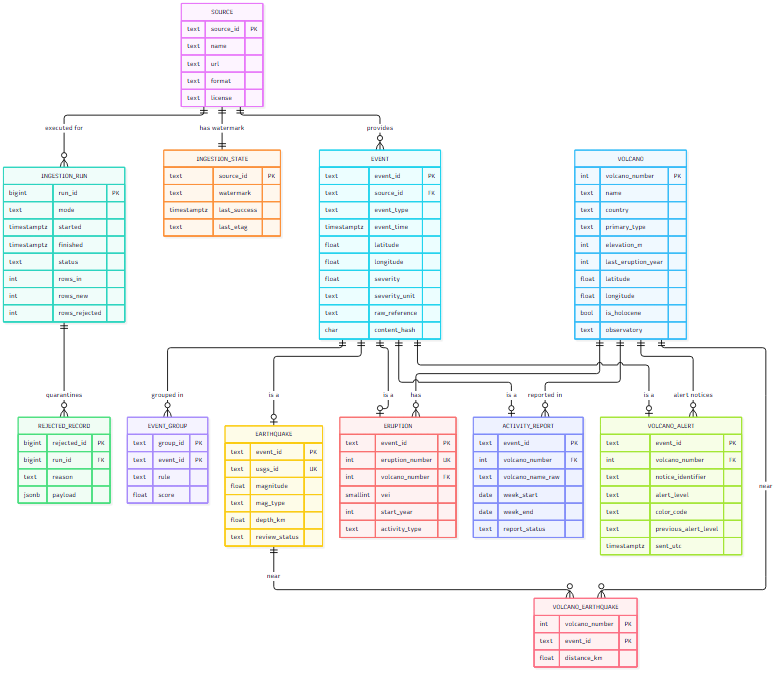
\includegraphics[width=\textwidth]{er_diagram.png}
\caption{First-draft ER diagram of the canonical model (source:
\texttt{docs/er\_diagram.mmd}). The upper block is the model required of every team;
\texttt{volcano} and the domain tables are specific to volcanic activity.}
\label{fig:er}
\end{figure}

%==============================================================================
\section{Ingestion Contract}
\label{sec:contract}

Each source has a historical strategy, an incremental strategy with a watermark, an
overlap window and a duplicate key (Table~\ref{tab:contract}). The full version is in
\texttt{workshop\_1/ingestion\_contract.md}; the same values are declared in
\texttt{config/sources.yaml}.

\begingroup
\footnotesize
\setlength{\tabcolsep}{3pt}
\begin{longtable}{@{}L{1.5cm}L{3.0cm}L{3.6cm}L{2.2cm}L{1.9cm}L{2.4cm}@{}}
\caption{Per-source ingestion contract.}
\label{tab:contract}\\
\toprule
\textbf{Source} & \textbf{Historical strategy} & \textbf{Incremental strategy} &
\textbf{Watermark} & \textbf{Overlap window} & \textbf{Duplicate key} \\
\midrule
\endfirsthead
\multicolumn{6}{@{}l}{\small\itshape Table \thetable{} -- continued from previous page}\\
\toprule
\textbf{Source} & \textbf{Historical strategy} & \textbf{Incremental strategy} &
\textbf{Watermark} & \textbf{Overlap window} & \textbf{Duplicate key} \\
\midrule
\endhead
\midrule
\multicolumn{6}{r@{}}{\small\itshape continued on next page}\\
\endfoot
\bottomrule
\endlastfoot

GVP volcanoes & One filtered WFS request (165 features) &
Monthly; reload when the database version changes & GVP database version & --- &
\texttt{Volcano\_Number} \\
\addlinespace
GVP eruptions & One WFS request for the full layer (11{,}089 features), US subset by
\texttt{Volcano\_Number} (1{,}281) &
Monthly; compare content hash per eruption (catches new end dates and VEI revisions) &
GVP version + row hash & --- & \texttt{Eruption\_Number} \\
\addlinespace
USGS FDSN & Radial query per volcano (30~km, M~$\geq$~1.0), 2010 $\rightarrow$ today,
165 volcanoes; split by year when \texttt{count} > 20{,}000 (Kilauea, Clear Lake) &
Daily \texttt{updatedafter=<watermark>} around the US volcanoes &
max committed \texttt{updated} & Re-query the last 7 days & \texttt{id} \\
\addlinespace
USGS HANS & Not historical: the first run loads the current notice of the $\sim$69
monitored volcanoes &
Hourly snapshot of \texttt{getMonitoredVolcanoes}; a
\texttt{(vnum, notice\_identifier)} pair not yet committed = new notice; compare with
the previous notice of the volcano to flag raised or lowered levels &
max committed \texttt{sent\_unixtime} (epoch s) &
Whole snapshot on every poll (69 rows, 45~KB) &
\texttt{(vnum, notice\_identifier)} \\
\addlinespace
USGS feed & Not historical (rolling 7 days); the FDSN load covers the past &
Every 15 min; keep features with \texttt{updated} > watermark, store those within
30~km of a US volcano with M~$\geq$~1.0 &
max committed \texttt{updated} (epoch ms) & The 7-day window overlaps every poll &
\texttt{id} (same as FDSN) \\
\addlinespace
Weekly report (optional) & Not available as an API (archive is HTML only) &
Every 6 h, conditional GET (\texttt{ETag} / \texttt{Last-Modified}); keep US items &
last committed \texttt{week\_end} & Whole feed re-read each poll &
\texttt{(vnum, week\_start)} \\
\end{longtable}
\endgroup

\paragraph{Correctness when a run fails halfway.}
\begin{itemize}
  \item Every response is saved unmodified to the raw landing zone
  (\texttt{data/raw/<source>\_YYYYMMDD\_HHMMSS.<ext>} + \texttt{.meta.json} with URL,
  headers and SHA-256) before processing. A failed run is re-processed from disk
  without calling the API again.
  \item Each source --- and each FDSN partition --- is loaded in one database
  transaction. Its \texttt{ingestion\_run} row moves from \texttt{running} to
  \texttt{success} or \texttt{failed}.
  \item The watermark is updated in the same transaction as the data. On failure
  everything rolls back and the watermark keeps its old value, so the next run repeats
  the same interval. If FDSN fails after 80 of 165 volcanoes, the next run repeats only
  the missing partitions.
  \item All writes are upserts on the duplicate key
  (\texttt{ON CONFLICT \dots{} DO UPDATE WHERE content\_hash} differs). Repeating an
  interval creates no duplicates, and running either mode twice gives identical counts.
  \item HTTP calls use timeouts (10~s connect / 120~s read) and up to four retries with
  exponential backoff (2, 4, 8, 16~s) on 429 and 5xx, honouring \texttt{Retry-After}.
\end{itemize}

\paragraph{Deletions.}
An earthquake that leaves the feed is not deleted. It is checked against FDSN and
marked \texttt{review\_status = 'deleted'} only if USGS reports it deleted. A replaced
HANS notice is kept as history in \texttt{volcano\_alert}; the current state comes from
the view.

%==============================================================================
\section{Functional User and User Stories}
\label{sec:user}

\paragraph{Functional user.}
A hazard analyst at a state emergency-management agency --- for example the Alaska
Division of Homeland Security \& Emergency Management or the Hawaii Emergency
Management Agency --- or at a FEMA regional office. This analyst is not a
volcanologist and does not run an observatory. Each week they brief decision makers on
which US volcanoes show unusual activity and how reliable that picture is.

\begin{itemize}
  \item \textbf{Profile:} comfortable with maps and charts, not with seismology;
  checks the dashboard daily, and right away when HANS publishes a raised alert level.
  \item \textbf{Decisions supported:} which volcanoes go on the weekly watch list,
  when to contact the USGS observatory (AVO, HVO, CVO, CalVO, YVO) for an official
  assessment, and which situations to escalate in the briefing --- for example an
  aviation colour code that reaches ORANGE near flight routes.
  \item \textbf{Why the dashboard helps:} it puts the official alert level, nearby
  seismicity and eruption history of each volcano in one place, says whether the
  current seismicity is unusual for that volcano, and shows how fresh and complete the
  data is. The official alert always comes from the USGS observatory, and the dashboard
  says so.
\end{itemize}

\paragraph{User stories.}
Prioritised with MoSCoW and covering the three required themes --- \emph{monitoring}
(what is new), \emph{analysis} (is this unusual?) and \emph{trust} (how fresh and how
complete is the data?) --- in Table~\ref{tab:stories}.

\begingroup
\small
\setlength{\tabcolsep}{4pt}
\begin{longtable}{@{}L{1.0cm}L{2.1cm}L{1.9cm}L{10.0cm}@{}}
\caption{User stories, by MoSCoW priority and area.}
\label{tab:stories}\\
\toprule
\textbf{\#} & \textbf{Priority} & \textbf{Area} & \textbf{User story} \\
\midrule
\endfirsthead
\multicolumn{4}{@{}l}{\small\itshape Table \thetable{} -- continued from previous page}\\
\toprule
\textbf{\#} & \textbf{Priority} & \textbf{Area} & \textbf{User story} \\
\midrule
\endhead
\midrule
\multicolumn{4}{r@{}}{\small\itshape continued on next page}\\
\endfoot
\bottomrule
\endlastfoot

US1 & Must & Monitoring &
As an emergency-management analyst, I want to see on a map the current USGS alert
level and colour code of every US volcano, with changes since the last poll
highlighted, so that I know what changed. \\
\addlinespace
US2 & Must & Monitoring &
As an emergency-management analyst, I want to list the earthquakes of the last 7~days
within 30~km of each volcano, so that I can see which volcanoes have recent
seismicity. \\
\addlinespace
US3 & Must & Analysis &
As an emergency-management analyst, I want each volcano's current weekly earthquake
count compared with its 2010--present baseline (percentile), so that I can tell
whether the activity is unusual for that volcano. \\
\addlinespace
US4 & Must & Trust &
As an emergency-management analyst, I want to see the last successful run, watermark
age and rejected-record count per source, so that I know how fresh and complete the
data is. \\
\addlinespace
US5 & Should & Analysis &
As an emergency-management analyst, I want a volcano's eruption history (dates, VEI)
next to its current indicator, so that I can put the current activity in context. \\
\addlinespace
US6 & Should & Monitoring &
As an emergency-management analyst, I want the Volcano Activity Indicator ranked for
all US volcanoes and filterable by region (Alaska, Hawaii, Cascades\dots), so that I
can build the weekly watch list quickly. \\
\addlinespace
US7 & Could & Analysis &
As an emergency-management analyst, I want the indicator's history for a volcano over
the past year, so that I can see whether unrest is building or fading. \\
\addlinespace
US8 & Could & Trust &
As an emergency-management analyst, I want each indicator to show which inputs were
available and their limitations, so that I do not over-interpret it. \\
\addlinespace
US9 & Won't (this semester) & Monitoring &
As an emergency-management analyst, I want e-mail alerts when a volcano's alert level
or indicator rises, so that I am notified without opening the dashboard. \\
\end{longtable}
\endgroup

%==============================================================================
\section{Volcano Activity Indicator (Preliminary)}
\label{sec:indicator}

The Volcano Activity Indicator (VAI) is a 0--100 score per volcano, recomputed after
each incremental run and kept weekly for history. It combines three components, each
scaled to $[0,1]$, and maps the result to four levels. It describes how active a
volcano currently looks compared with its own past. \textbf{It does not estimate the
probability of an eruption.}

\begin{equation}
\mathrm{VAI} \;=\; 100 \cdot
\frac{w_R\,R + w_S\,S + w_H\,H}{\displaystyle\sum_{\text{available}} w}
\label{eq:vai}
\end{equation}

\begin{table}[h]
\centering
\small
\setlength{\tabcolsep}{5pt}
\caption{Components of the Volcano Activity Indicator.}
\label{tab:vai}
\begin{tabular}{@{}L{2.6cm}L{3.6cm}L{6.9cm}L{1.9cm}@{}}
\toprule
\textbf{Component} & \textbf{Input} & \textbf{Rule} & \textbf{Default weight} \\
\midrule
$R$ --- reported activity &
USGS HANS alert level (optional bonus from the weekly report) &
NORMAL 0, ADVISORY 0.4, WATCH 0.7, WARNING 1.0; $+0.2$ if the volcano is NEW in the
latest weekly report, $+0.1$ if continuing; capped at 1.0. The colour code is shown,
not scored separately &
$w_R = 0.45$ \\
\addlinespace
$S$ --- seismic anomaly &
Earthquakes M~$\geq$~1.0 within 30~km (FDSN baseline + feed) &
$p$ = percentile of the last-7-day count within the volcano's own weekly counts since
2010; $S = \max\!\left(0, (p - 0.5)/0.5\right)$. $S$ is ``not available'' when the
volcano has fewer than 20 baseline earthquakes &
$w_S = 0.35$ \\
\addlinespace
$H$ --- eruptive state &
GVP eruptions &
1.0 if an eruption has no end date; else
$\exp\!\left(-\,\Delta t / 25\right)$ with $\Delta t$ in years since the last eruption &
$w_H = 0.20$ \\
\bottomrule
\end{tabular}
\end{table}

\noindent
\textbf{Levels:} LOW $<25\leq$ MODERATE $<50\leq$ ELEVATED $<75\leq$ HIGH. Weights,
alert-level scores, radius, minimum magnitude, decay constant and thresholds are
parameters in \texttt{config/sources.yaml} (\texttt{indicator:} block), not constants
in code. A component that is not available is dropped and the remaining weights are
renormalised, which is why the denominator of equation~\eqref{eq:vai} sums only the
available weights; the dashboard shows which components were used (US8).

\subsection{Validation against historical events}

\begin{itemize}
  \item Rebuild a weekly VAI history from 2010 with the $S$ and $H$ components only.
  $R$ cannot be back-filled, because HANS returns only the latest notice per volcano;
  it accumulates from the first poll.
  \item For every GVP eruption since 2010 at US volcanoes with an adequate seismic
  baseline, check whether the VAI was ELEVATED or HIGH in the four weeks before or
  after the start date (hit rate). Measure how often it is ELEVATED in weeks with no
  eruption (false-alarm rate).
  \item Case studies:
  \begin{itemize}
    \item \textbf{Kilauea}, 2018 lower East Rift Zone eruption: dense HVO network,
    expected to be detected.
    \item \textbf{Mauna Loa}, November 2022 eruption, preceded by weeks of increased
    seismicity: expected to be detected.
    \item \textbf{Great Sitkin}, eruption starting 2021-05-25 (GVP 22401): an Aleutian
    volcano with a smaller network, a test of the baseline rule.
    \item \textbf{Ahyi Seamount} (CNMI), eruption starting 2025-10-20: submarine with
    sparse seismic coverage, expected to be missed by $S$. This illustrates the
    limitation.
  \end{itemize}
  \item Sensitivity analysis: vary the radius (15/30/50~km), the minimum magnitude and
  the weights, and report how the hit and false-alarm rates change.
\end{itemize}

\subsection{Limitations}

\begin{itemize}
  \item $S$ depends on the local network: well-instrumented volcanoes (Hawaii,
  Cascades) have a usable baseline; remote Aleutian and Mariana volcanoes may not.
  \item Clear Lake, The Geysers area and other geothermal fields produce many
  non-volcanic earthquakes, so a 30~km count can be high without any volcanic unrest.
  \item $R$ reflects official alert levels, which change in discrete steps and can lag
  the data.
  \item VEI and eruption dates are uncertain for older eruptions; VEI is missing for
  37.5\,\% of the US eruptions.
  \item One earthquake within 30~km of two volcanoes raises the component of both.
  This is intended, not double counting: 435 distinct identifiers in the FDSN sample
  are in that situation.
  \item The VAI is a relative, descriptive monitoring aid. Official alert levels come
  from the USGS volcano observatories.
\end{itemize}

%==============================================================================
\section{Risks and Mitigation}
\label{sec:risks}

Table~\ref{tab:risks} lists ten risks. R2, R3, R5, R6 and R8 were \emph{directly
observed} while validating the sources on 2026-11-10 and 2026-11-11 and are recorded
in \texttt{workshop\_1/source\_status\_log.md}. R7 and R9 are documented behaviour of
the sources for which the samples already show evidence. R1, R4 and R10 are
anticipated risks inherent to the design rather than incidents observed so far.

\begingroup
\footnotesize
\setlength{\tabcolsep}{4pt}
\begin{longtable}{@{}L{0.7cm}L{3.4cm}L{1.6cm}L{1.3cm}L{7.5cm}@{}}
\caption{Project risks, with likelihood, impact and mitigation.}
\label{tab:risks}\\
\toprule
\textbf{\#} & \textbf{Risk} & \textbf{Likelihood} & \textbf{Impact} &
\textbf{Mitigation} \\
\midrule
\endfirsthead
\multicolumn{5}{@{}l}{\small\itshape Table \thetable{} -- continued from previous page}\\
\toprule
\textbf{\#} & \textbf{Risk} & \textbf{Likelihood} & \textbf{Impact} &
\textbf{Mitigation} \\
\midrule
\endhead
\midrule
\multicolumn{5}{r@{}}{\small\itshape continued on next page}\\
\endfoot
\bottomrule
\endlastfoot

R1 & Source outage (GVP GeoServer, HANS or the USGS feed down during a run or the
demo) & Medium & High &
Retries with backoff; the run is marked \texttt{failed} and the watermark is not
advanced; the raw landing zone and the recorded fixtures allow re-processing and an
offline demo \\
\addlinespace
R2 & Rate limits / 20{,}000-event cap on FDSN & Medium & Medium &
\texttt{count} before each query, split by year (Kilauea, Clear Lake), 1 request/s,
cache everything; never re-download the historical archive needlessly \\
\addlinespace
R3 & Schema or endpoint change (WFS field renamed, HANS endpoint moved, RSS format
changed) & Medium & High &
Parsers validate required fields and fail loudly; unparseable records go to
quarantine; HANS has a second endpoint (\texttt{getElevatedVolcanoes}) to cross-check;
changes are logged in \texttt{workshop\_1/source\_status\_log.md} and reported to the
professor. Already seen: the RSS \texttt{<link>} became generic and the eruption layer
has no lat/lon properties \\
\addlinespace
R4 & Licence and attribution (GVP requires version + DOI) & Low & Medium &
Citation and version stored in \texttt{config/sources.yaml}, shown in the dashboard
footer and in this report; the GVP version is recorded with each load \\
\addlinespace
R5 & Data volume (365{,}100 FDSN rows; Kilauea alone 87{,}679) & Medium & Medium &
Partition by volcano and year; PostGIS indexes; store only feed events within 30~km of
a US volcano \\
\addlinespace
R6 & Ambiguous identifiers (placeholder vnums \texttt{0} / \texttt{999999}, region rows
without vnum, notices shared by several volcanoes, one earthquake near two volcanoes) &
High & Medium &
Link by \texttt{vnum} only; validation rules quarantine invalid vnums;
\texttt{(vnum, notice\_identifier)} as the HANS key; many-to-many
\texttt{volcano\_earthquake} table \\
\addlinespace
R7 & HANS keeps only the latest notice, so the alert history cannot be loaded backwards
& High & Medium &
Store every notice from the first poll; validate the indicator with $S$ and $H$ only
for past years; state the limitation \\
\addlinespace
R8 & Sparse incremental changes in HANS (one new notice in 44~h) give little to
demonstrate & Medium & Low &
Pair it with the minute-level USGS feed (636 new events in the same 44~h); keep
recorded snapshots as fixtures \\
\addlinespace
R9 & Records revised or withdrawn after publication (FDSN revises magnitude, location
and status and can delete events; GVP assigns end dates and can discredit eruptions) &
High & Medium &
\texttt{content\_hash} per row detects a changed record and updates it instead of
duplicating it; FDSN re-queries the last 7 days with \texttt{updatedafter}; absence
from the feed is confirmed against FDSN before marking a record deleted \\
\addlinespace
R10 & Over-claiming: a numeric indicator next to a map invites the reader to interpret
it as a forecast & Medium & High &
The VAI is named and documented as a monitoring aid; its three components are always
shown separately; the official USGS alert level is displayed next to it without
modification; the limitations of Section~\ref{sec:indicator} appear in the dashboard
itself \\
\end{longtable}
\endgroup

%==============================================================================
\section{Architecture Overview and Repository}
\label{sec:architecture}

The system follows the course reference architecture: sources $\rightarrow$ raw landing
zone $\rightarrow$ normalise/validate/deduplicate $\rightarrow$ canonical database
$\rightarrow$ analytics $\rightarrow$ dashboard, with a quarantine branch
(Figure~\ref{fig:architecture}). Everything runs locally with Docker Compose.

\begin{figure}[h]
\centering
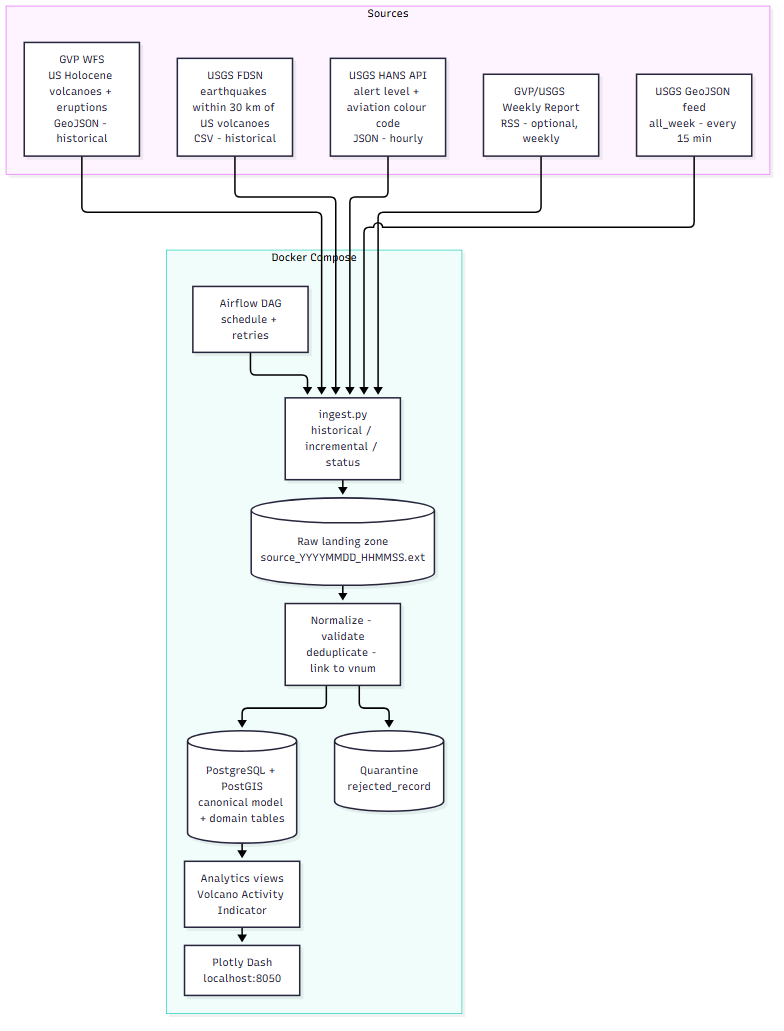
\includegraphics[width=\textwidth]{architecture.png}
\caption{Reference architecture adapted to volcanic activity (source:
\texttt{docs/architecture.mmd}).}
\label{fig:architecture}
\end{figure}

\noindent
Airflow triggers \texttt{ingest.py} on each source's schedule: hourly for HANS, every
15~minutes for the feed, daily for FDSN and monthly for GVP. Every response lands
unmodified in the raw zone before validation, and only validated rows reach
PostgreSQL/PostGIS. The dashboard reads exclusively from the database and its
analytical views.

\paragraph{Repository.}
\url{https://github.com/jhonatanvj/Proyecto_Analisis_De_Datos}

\begin{itemize}
  \item \texttt{ingest.py}: CLI stub with
  \texttt{-{}-mode historical|incremental|status}; \texttt{status} already lists
  sources, watermark fields and raw files.
  \item \texttt{src/volcano\_pipeline/}: \texttt{sources/} (HTTP clients with retries
  for GVP, FDSN, the feed, HANS and the weekly RSS), \texttt{normalization/}
  (canonical mappers, geo helpers), \texttt{storage/} (raw landing zone).
  \item \texttt{config/sources.yaml}: one entry per source with URL, format, schedule,
  watermark field, duplicate key, licence and citation, plus the indicator parameters.
  \item Other folders: \texttt{data/raw/} (git-ignored), \texttt{sql/} (draft DDL),
  \texttt{dashboard/} (placeholder), \texttt{tests/} and \texttt{tests/fixtures/}
  (16 passing pytest tests, two of them on recorded HANS and RSS responses, no live
  calls), \texttt{notebooks/01\_source\_profiling.ipynb}, \texttt{docs/},
  \texttt{workshop\_1/} (mapping, contract, samples, source status log).
  \item Root files: \texttt{scripts/fetch\_samples.py}, \texttt{.env.example},
  \texttt{.gitignore}, \texttt{requirements.txt} and \texttt{README.md}. No API keys
  are needed, and \texttt{.env} is never committed.
\end{itemize}

\begin{table}[h]
\centering
\small
\setlength{\tabcolsep}{5pt}
\caption{Location of each Workshop~\#1 deliverable in the repository.}
\label{tab:deliverables}
\begin{tabular}{@{}L{5.0cm}L{10.0cm}@{}}
\toprule
\textbf{Deliverable} & \textbf{Location} \\
\midrule
Project definition report & \texttt{docs/project\_definition.tex} (this document) \\
Source profiling notebook & \texttt{notebooks/01\_source\_profiling.ipynb} \\
Raw evidence samples & \texttt{workshop\_1/samples/} (unmodified responses with SHA-256 sidecars) \\
Canonical mapping table & \texttt{workshop\_1/mapping.md} and \texttt{workshop\_1/mapping.csv} \\
Ingestion contract & \texttt{workshop\_1/ingestion\_contract.md} \\
Source status log & \texttt{workshop\_1/source\_status\_log.md} \\
ER diagram and architecture & \texttt{docs/er\_diagram.png}, \texttt{docs/architecture.png} \\
Draft schema & \texttt{sql/001\_schema\_draft.sql} \\
Source configuration & \texttt{config/sources.yaml} \\
CLI entry point & \texttt{ingest.py} \\
Tests and fixtures & \texttt{tests/}, \texttt{tests/fixtures/} \\
\bottomrule
\end{tabular}
\end{table}

%==============================================================================
\section{References}
\label{sec:references}

\begin{itemize}[leftmargin=0.6cm]
  \item Global Volcanism Program, 2026. \emph{[Database] Volcanoes of the World}
  (v.~5.4.0; 7~Aug~2026). Distributed by Smithsonian Institution, compiled by
  Venzke,~E. \url{https://doi.org/10.5479/si.GVP.VOTW5-2026.5.4}

  \item Smithsonian GVP, \emph{Volcanoes of the World Webservices} (WFS layers,
  formats, citation).
  \url{https://webservices.volcano.si.edu/geoserver/GVP-VOTW/ows}

  \item U.S. Geological Survey, Volcano Hazards Program, \emph{Hazard Notification
  System (HANS) public API}. \url{https://volcanoes.usgs.gov/hans-public/api}

  \item U.S. Geological Survey, Volcano Hazards Program, \emph{Volcano Alert Levels and
  Aviation Color Codes}.

  \item U.S. Geological Survey, Earthquake Hazards Program, \emph{FDSN Event Web
  Service, ANSS Comprehensive Earthquake Catalog (ComCat)}.
  \url{https://earthquake.usgs.gov/fdsnws/event/1/}

  \item U.S. Geological Survey, Earthquake Hazards Program, \emph{Real-time GeoJSON
  Summary Feeds}.
  \url{https://earthquake.usgs.gov/earthquakes/feed/v1.0/geojson.php}

  \item Global Volcanism Program, \emph{Smithsonian / USGS Weekly Volcanic Activity
  Report}, Sennert,~S. (ed.) (optional source).

  \item Newhall, C.~G., and Self, S. (1982). The Volcanic Explosivity Index (VEI): An
  estimate of explosive magnitude for historical volcanism. \emph{Journal of
  Geophysical Research}, 87(C2), 1231--1238.

  \item Course documents: \emph{Course Project Description} and \emph{Workshop No.~1},
  Data Analysis Programming 2026-II, Eng. Carlos Andr\'es Sierra, Universidad Distrital
  Francisco Jos\'e de Caldas.
\end{itemize}

\bigskip
\noindent
\small
USGS products are in the public domain and are credited to the U.S. Geological Survey.
Smithsonian GVP data are used under the Global Volcanism Program terms of use, citing
the database version and DOI as required. No source used in this project requires an
API key, and no credential is stored in the repository.

\end{document}
